\documentclass[letterpaper,notitlepage,twoside]{article}

% Basic imports, increase margins...
\usepackage[margin=0.75in]{geometry}
% Finite State Machine stuff
\usepackage{pgf}
\usepackage{tikz}
\usetikzlibrary{arrows, automata}
% Format tables nicely
\usepackage[latin1]{inputenc}
\usepackage{array}

\usepackage{amsfonts}
\usepackage{amssymb}
\usepackage{amsmath,amsthm}

\renewcommand{\implies}{\Rightarrow} % redefine command "implies"
\renewcommand{\iff}{\Leftrightarrow} % double arrow
\newcommand{\maps}{\rightarrow} % define command "map"
\newcommand{\union}{\cup}
\newcommand{\intersect}{\cap}
\newcommand{\N}{\mathbb{N}} % natural number
\newcommand{\Q}{\mathbb{Q}} % rational number
\newcommand{\R}{\mathbb{R}} % real number
\newcommand{\Z}{\mathbb{Z}} % integers
\newcommand\tab[1][1cm]{\hspace*{#1}} %\tab command

% Add more packages that you use here...

\begin{document}
\title{Homework 25}
\author{Brian Knotten, Brett Schreiber, Brian Falkenstein}
\maketitle
\subsection*{19}
In the given crossing gadget $G$, the vertices $x$ and $x'$ must be the same color for all 3-colorings of $G$. This is proved via contradiction. Assume $x$ and $x'$ could be colored two different colors in a valid 3-coloring $G$. Then the graph $H$, which is identical to $G$ except for an extra edge $(y, y')$ could also be 3-colorable, since $y$ and $y'$ could just be the two different colors. In other words, an extra edge wouldn't affect the colorability if $x$ and $x'$ were able to be two different colors.
\\
First, a triangle within $H$ was arbitrarily chosen to be colored $1, 2, 3$ (denoted by bold edges below). Any other 3-color attempts can be converted into this canonical form by swapping colors within the triangle. For most of the coloring, vertices were forced to be a certain color due to their neighbors. There was only one point where a vertex had a choice of two different colors, which is why we present two graph colorings (differences denoted by bold vertices below). Both canonical graph colorings lead to having a vertex $v$ that is adjacent to all three colors, in which case it can be deemed impossible to 3-color $H$, contradicting our assumption. Below are the two graph colorings of $H$:
\\\\
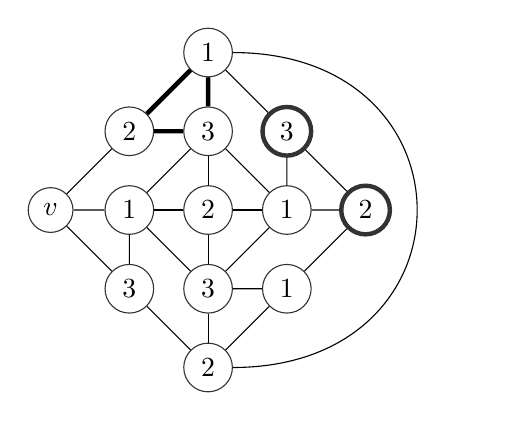
\begin{tikzpicture}
    \node[circle,draw=black!80] (a) at (0, 1) {$v$};
    \node[circle,draw=black!80] (b) at (1, 1) {$1$};
    \node[circle,draw=black!80] (c) at (2, 2) {$3$};
    \node[circle,draw=black!80] (d) at (2, 0) {$3$};
    \node[circle,draw=black!80] (e) at (3, 1) {$1$};
    \node[circle,draw=black!80] (f) at (2, 1) {$2$};
    \node[circle, ultra thick, draw=black!80] (g) at (4, 1) {$2$};
    \node[circle,draw=black!80] (h) at (1, 2) {$2$};
    \node[circle,draw=black!80] (i) at (1, 0) {$3$};
    \node[circle, ultra thick ,draw=black!80] (j) at (3, 2) {$3$};
    \node[circle,draw=black!80] (k) at (3, 0) {$1$};
    \node[circle,draw=black!80] (l) at (2, 3) {$1$};
    \node[circle,draw=black!80] (m) at (2, -1) {$2$}; 
    \draw (a) -- (b) -- (c) -- (e) -- (g);
    \draw (b) -- (d) -- (e);
    \draw (b) -- (f) -- (e);
    \draw (c) -- (f) -- (d);
    \draw (a) -- (h) -- (c);
    \draw (a) -- (i) -- (b);
    \draw (h) -- (l) -- (j) -- (e);
    \draw (l) -- (c);
    \draw (j) -- (g);
    \draw (d) -- (k) -- (g);
    \draw (i) -- (m) -- (k);
    \draw (d) -- (m);
    \draw [ultra thick] (h) -- (l) -- (c) -- (h);
    %\draw [ultra thick] (a) -- (b) -- (i) -- (a);
   % \draw [ultra thick] (e) -- (g) -- (j) -- (e);
    %\draw [ultra thick] (d) -- (m) -- (k) -- (d);
    \path (l) edge[bend left=90, looseness=2] node [left] {} (m);
\end{tikzpicture}
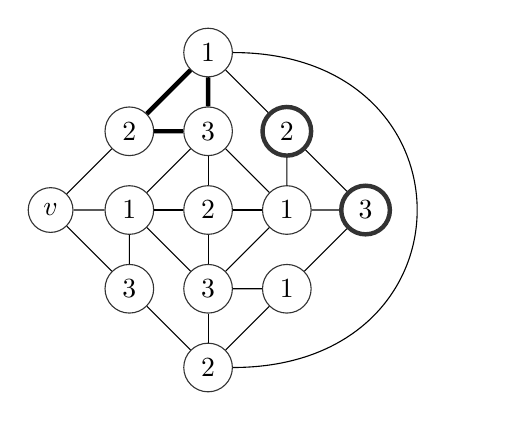
\begin{tikzpicture}
    \node[circle,draw=black!80] (a) at (0, 1) {$v$};
    \node[circle,draw=black!80] (b) at (1, 1) {$1$};
    \node[circle,draw=black!80] (c) at (2, 2) {$3$};
    \node[circle,draw=black!80] (d) at (2, 0) {$3$};
    \node[circle,draw=black!80] (e) at (3, 1) {$1$};
    \node[circle,draw=black!80] (f) at (2, 1) {$2$};
    \node[circle, ultra thick, draw=black!80] (g) at (4, 1) {$3$};
    \node[circle,draw=black!80] (h) at (1, 2) {$2$};
    \node[circle,draw=black!80] (i) at (1, 0) {$3$};
    \node[circle, ultra thick, draw=black!80] (j) at (3, 2) {$2$};
    \node[circle,draw=black!80] (k) at (3, 0) {$1$};
    \node[circle,draw=black!80] (l) at (2, 3) {$1$};
    \node[circle,draw=black!80] (m) at (2, -1) {$2$};
    \draw (a) -- (b) -- (c) -- (e) -- (g);
    \draw (b) -- (d) -- (e);
    \draw (b) -- (f) -- (e);
    \draw (c) -- (f) -- (d);
    \draw (a) -- (h) -- (c);
    \draw (a) -- (i) -- (b);
    \draw (h) -- (l) -- (j) -- (e);
    \draw (l) -- (c);
    \draw (j) -- (g);
    \draw (d) -- (k) -- (g);
    \draw (i) -- (m) -- (k);
    \draw (d) -- (m);
    \draw [ultra thick] (h) -- (l) -- (c) -- (h);
    %\draw [ultra thick] (a) -- (b) -- (i) -- (a);
    %\draw [ultra thick] (e) -- (g) -- (j) -- (e);
    %\draw [ultra thick] (d) -- (m) -- (k) -- (d);
    \path (l) edge[bend left=90, looseness=2] node [left] {} (m);
\end{tikzpicture}
\\\\
Since $G$ is symmetrical, it is also the case that $x$ and $x'$ must be colored the same color for all 3-colorings of $G$. Consider the graph $G'$ identical to $G$ except with two more vertices, $x''$ and $y''$, and two more edges, $(x', x'')$ and $(y', y'')$. It must be the case that $y'$ and $y''$ must be different colors in all 3-colorings of $G'$, since they share an edge, and the same reasoning applies for $x'$ and $x''$. Furthermore, it must be the case that $y$ and $y''$ must be different colors, since the color of $y$ is the same as the color of $y'$, which is different from the color of $y''$. Again, the same reasoning applies to $x$ and $x''$.
\\
Now we can reduce 3-Color to Planar 3-Color. For every crossing in 3-Color's input graph between four vertices, $x, x'', y, y''$ replace the crossing with the subgraph $G'$ described above. Now there is no longer an edge directly between $x$ and $x''$ or $y$ and $y''$, but the property that both pairs must be colored two different colors remains. Moreover, the crossing has been removed. Repeat this process for all crossings to obtain a planar graph $P$. Run the Planar 3-Color algorithm on $P$ to obtain a 3-Coloring.

\subsection*{21}
Define the problem described as VDP (vertex disjoint paths). In order to show that $3SAT \geq _{poly} VDP$, we will first show that $VDP$ is self reducible. That is, given the decision problem for VDP, we can determine the paths connecting each $(s_i, t_i)$. \\\\
$VDP_{opt} \geq _{poly} VDP_{decision}$\\\\
Given as input to $VDP_{opt}$ a graph $G$ and a set of tuples $(s_1, t_1) ... (s_n, t_n)$, we can use the decision problem $VDP_{decision}$ to get the actual paths from each $s_i$ to each $t_i$. Define $P_i$ to be the path connecting $s_i$ to $t_i$. \\
First check if $VDP_{decision}$ on $G$ and $(s_1, t_1) ... (s_n, t_n)$ returns 1. If not, then paths don't exist. If 1, use breadth first search to get all neighbors of $s_1$, call these $v_1...v_k$. Now, call $VDP_{decision}$ on $G$ and $(v_i, t_1) ... (s_n, t_n)$ for $1\leq i \leq k$. If this returns 1, add $v_i$ to the path for $(s_1, t_1)$ $P_1$ and continue this process, searching for neighbors of $v_i$, etc. \\
Note that for each vertex added to a path $P_i$, we must make sure that that vertex does not appear in any other paths. We can enforce this by adding a new tuple to the input. If $v_i$ was the vertex added to the path for some $(s_i, t_i)$, then construct a new $(s, t)$ to be $(v_i, v_i)$. Since the shortest path from $v_i$ to $v_i$, it will always be an option to have its path be just $v_i$. This forces other subsequent paths to not include $v_i$. If we continue this process for all $k$ tuples, we will have the paths for all the inputs. \\
This transformation is poly time. For each tuple, we must perform BFS to get from $s_i$ to $t_i$, making one call to $VDP_{decision}$ at each point. Since BFS takes polynomial time in the number of vertices and edges in a graph ($O(|V| + |E|)$, in the worst chase, as all vertices and edges will be visited), and the number of edges is bound by the number of vertices (max E = $V^2$), if we say the number of vertices is $n$, than the time for each tuple will be $O(n^2)$. Doing this for all $k$ tuples gives us $(O(kn^2))$, where $k$ can be no larger than $n/2$ (pigeonhole principle, since we cannot repeat vertices, if each vertex in $G$ were assigned to either a source or a sink). Thus, if a polynomial time algorithm exists for $VDP_{decision}$, than one exists for $VDP_{opt}$. \\\\
$3SAT \geq _{poly} VDP_{opt}$\\\\
Since we have shown that $VDP_{opt} \geq _{poly} VDP_{decision}$, if we have a poly-time algorithm for $VDP_{opt}$, than we also have a poly-time algorithm for 3SAT (IE, if we assume we have a polynomial time algorithm for decision, than we have one for opt). \\
We will show how to construct an instance of VDP from an instance of 3SAT, such that the VDP instance is true if and only if the 3SAT instance is satisfiable. To model choosing a variable $x$ in 3SAT as either true or false, construct the following sub-graph: \\
$$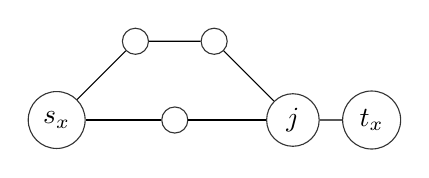
\begin{tikzpicture}
    \node[circle,draw=black!80] (a) at (0, 1) {$s_x$};
    \node[circle,draw=black!80] (b) at (1, 2) {};
    \node[circle,draw=black!80] (c) at (2, 2) {};
    \node[circle,draw=black!80] (d) at (1.5, 1) {};
    \node[circle,draw=black!80] (e) at (3, 1) {$j$};
    \node[circle,draw=black!80] (f) at (4, 1) {$t_x$};
    \draw (a) -- (b) -- (c) -- (e) -- (f);
    \draw (a) -- (d) -- (e);
\end{tikzpicture}$$
Here, there are 2 possible paths from $s_x$ to $t_x$, one of length 3 and one of length 4. Due to node $j$ being a bottleneck, only one of these paths can exist in the final output (as $j$ must be a member of both paths, they could not be disjoint). Take the path of length 3 being chosen to mean set $x$ to true, and the path of length $4$ being chosen to mean setting $x$ to false (or, setting $\overline x$ to true). Construct one such subgraph for each variable in the 3SAT instance. \\
Now, we must model the clauses in the 3SAT instance. That is, if the 3SAT formula is satisfiable, we will construct a subgraph that asserts that at least one of the literals in that clause will be true. We will construct some component $D$ for each clause. 

\end{document}
